\documentclass[11pt]{article}


\usepackage[]{graphicx}
\usepackage{natbib}
\usepackage{rotating}
\usepackage{subfloat}
\usepackage{pgfgantt}
\usepackage[margin=2cm]{geometry}

%opening
\title{Developing a train booking chatbot: Final report}
\author{Group 2M: Alvin Lu, Joe Newman and YuTing Liu}


\begin{document}

\maketitle

\section{Introduction}
According to \citet{Oracle}, Chat-bots are computer programmes that can simulate and process natural language conversation with humans. Chatbot has received major increase in popularity for organisations recently due to its capability to resolve tasks using natural language with greater efficiency relative to a human operator. While general (conversational) chatbot exists and are able to respond and process a wide range of conversation and instructions, most chatbots that are developed are specialised in a certain task. The aim of this project is to develop a task-oriented chatbot that can locate the cheapest train ticket given the details, predict train delays for selected train routes and provide contingencies for experts during a train journey.

\subsection{Background and Motivation}
Chatbots was first introduced in the 1960s. Initially, chatbots were developed with the goal to mimic natural conversation (of a specific group of individual) without any specific goals or tasks to be accomplished. Some notable early chatbots are ELIZA, PARRY which uses simple systems such as response pairing. Another major development was the growth of chatbots that uses pattern matching instead of pairing pre-defined response pairs. The classic example of such chatbot is Jabberwocky, which has been used for academic research. Chatbots grew significantly in popularity in the early 2000s, organisations are developing task-oriented chatbots to handle specific tasks online. General purpose chatbots such as Siri, Google assistant and Alexa became more common this decade. These chatbots have a ability to process and handle large amount of different tasks.

Chatbots provide various advantages to the operations of an organisation, and with the increase of platforms and open-source programs that aids the development of chatbot, the amount of chatbots deployed online has been growing significantly. Unlike human customer support, Chatbots are able to process multiple user request in parallel and are always available any time of the day \citep{ChatBotPros}. Chatbots can also engage customer proactively to engage with customers, collecting and monitoring customer data during the process. More advanced chatbot can also improve the organisations presence in the global market by providing chatbots in different languages. Some online platforms also allow chatbots to be deployed to other platforms such as social media which would further increase the amount of engagement an organisation has on its market \cite{ChatBotPros}.

There are also certain limitations on chatbots as well. Task-oriented chatbots are usually constrained in the type of conversations it could process, conversation that went out of scope might result in \citep{ChatBotProsCons}:
\begin{itemize}
	\item Default response when chatbots fail to process the conversation
	\item Inaccurate assumption of users intention, causing problems in communication
\end{itemize}
Whilst it's possible to develop chatbots that are capable of handling large amount of tasks, it's time consuming and costly to deploy such chatbot that may not be utilised fully. Therefore, an additional objective of this project is to develop a chatbot that is capable of handling most conversation within the scope of the tasks while providing relevant information when the conversation goes out of scope.

\subsection{Components of a Chatbot}
There are multiple different components in the background that simulates natural language conversation in a task-oriented chatbot.
\subsubsection{Natural language processing}
Natural language processing (NLP) is a crucial part of a chatbot as it functions as the connection between natural language conversation to the background functionalities. NLP functions to process sentences that user entered and extract the intentions of the user \citep{NLPIntro}. Two of the main method of understanding natural sentences: Syntactic analysis works by applying grammatical rules and grouping words in sentences to derive meaning from the sentence. On the other hand, Semantic analysis aims to derive meaning of words by trying to understand the meaning of words by analysing the sentence, context and grammar \citep{NLPIntro}.

\subsubsection{Reasoning engine}
While NLP processes and understands the meaning of a sentence, a reasoning engine is responsible mapping the extracted meaning to actions. It uses defined rules or models to discover the aim or intent of the user and provides relevant responses accordingly.

\subsubsection{Web Scraping}
Web-scraping is the process of extracting structured data from the web for other processes. The module can go through a webpage and extract information that is required. Web scrapers also has the ability to submit and fill in information online as well to request for further information such as automatically filling in a form. Web scraping is an important component for a train booking chatbot as well because information about train tickets has to be obtained online.

\subsubsection{Data mining}
Data mining is the act of extracting previously unknown information from data and converting into a structured format for other uses. The purpose of data mining is to discover pattern, anomalies or correlations. Data mining is usually done on combination with other aspects of computing such as AI, Statistics and Machine learning and the information obtained would be used for some other operations.

\subsubsection{Predictive model}
A predictive model provides forecast of certain outcomes. A predictive model is usually trained with existing structured data using a specified method or a combination of different method and makes a forecast based on the data it's trained on. For the train booking chatbot, it will be trained on previous train delay data and provide predictions on delays of new unseen train delays. 

\subsubsection{Knowledge-base system}
Knowledge-base system contains a collection of information that can be accessed using an inference engine. These information is typically used as part of a decision making process and for the chatbot, it will be used to save information regarding actions to take in case of an emergency.

\section{Methods, Tools and Frameworks}
\subsection{Methods}
As there as multiple different components for a chatbot, the components will be developed separately with clear requirements set for each of the components to decrease the amount of bugs that may occur during the combination of different components. Team members will be assigned with 1 to 3 components that are linked to develop, with constant updates on the progress

\subsubsection{Code management}
As components will be developed independently, all codes will be uploaded to GitHub repository. Compilation and error checking will be assigned to one member. Each member will create a separate branch for code development and codes will be merged after a meeting with the full team.
             
\subsection{Languages, Packages, Tools}

\subsubsection{Language}
Following the requirement, the chatbot will be developed mainly in \textit{Python}. \textit{Python} contains a vast library of packages and framework that supports the development of an intelligent system which will significantly reduce the amount of time needed for development. Aside from that, the User interface will be developed using HTML and CSS and supported by \textit{Flask}.

\subsubsection{Packages}
For Natural language processing, there are two packages that can be used to support the development: \textit{SpaCy} and \textit{NLTK}. Both packages allow tokenises and groups words together using a model that it was trained on. These packages can be used to assist in extracting information needed for the different tasks especially location and intent. For the current implementation, database can be developed in \textit{SQLite} as it provides a quick implementation of a full SQL engine. This will allow execution of a database without a working server.

Prediction model can be created and tested using the \textit{Sci-kit learn} package. With the support from \textit{Numpy} for data pre-processing and \textit{Joblib} file format for storage of models, Various different models can be created and tested with our dataset and models trained can be saved permanently without the need of retraining. In terms of historical train data, the \textit{HSP} API provides an intensive record of historical train data which can be retrieved using an account for the API. There are several packages available for knowledge-base such as pyke however \textit{Experta} provides a relatively simpler syntax for a rule-based inference system. \textit{Experta} is a branch of the \textit{pyKnow} package and uses the same format as its predecessor.

Website scraping can be achieved by utilising \textit{Scrapy}, \textit{BeautifulSoup} and \textit{Selenium}. \textit{Scrapy} implements web crawlers called "Spiders" that are contained within a class. Each spider are specialised in the information they scrape online. \textit{BeautifulSoup} has similar functions in which they can scrape html for information but \textit{Selenium} is capable of interacting with a webpage such as completing forms and clicking buttons.

\subsubsection{Tools}
The chatbot will be developed using \textit{Visual Studio Code}, a code editor that allows development of python software and it also includes packages for error checking and syntax highlighting. Visual studio code also allows editing of other file types such as \textit{HTML}, \textit{CSS} and \textit{csv} files all with error checking and syntax highlighting available. In terms of database management, DB Browser is a software that allows viewing and managing of data. Having a database management software allows testing whether if database interaction is successful between modules and also allow manual analysis of collected data.

\subsection{Work Plan}
\begin{sideways}
	\begin{ganttchart}[x unit=0.264 cm, y unit chart = 0.55 cm, vgrid, title label font=\scriptsize,canvas/.style={draw=black, dotted}]{1}{70} \label{gantt}
		\gantttitle[x unit=2.31cm]{Work plan for developing Chat-bot shown in semester week numbers}{8} \\
		\gantttitlelist[x unit=1.848cm]{8,...,17}{1} \\
		\gantttitlelist[x unit=0.264cm]{1,...,70}{1} \\
		\ganttgroup{Research}{1}{21}\\
		\ganttbar{Background research}{1}{5} \\
		\ganttbar{Analyse current systems}{1}{5} \\
		\ganttlinkedbar{Draft specification}{6}{10} \\
		\ganttbar{Package review}{1}{5} \\
		\ganttlinkedbar{Test/ Setup packages}{6}{17} \ganttnewline
		\ganttlinkedbar{Write report}{18}{65} \ganttnewline
		\ganttbar{Allocate components}{18}{20} \\
		\ganttmilestone{Initial design}{21} \ganttnewline
		
		\ganttgroup{Development}{22}{50}\\
		\ganttbar{Prototyping}{22}{50} \\
		\ganttbar{NLP}{22}{32} \\
		\ganttlinkedbar{Reasoning engine}{33}{50} \\
		\ganttbar{Data mining}{22}{30} \\
		\ganttlinkedbar{Prediction model}{31}{50} \\
		\ganttbar{Database}{22}{35} \\
		\ganttlinkedbar{Web scraper}{36}{45} \\
		\ganttlinkedbar{UI}{46}{50} \\
		\ganttlinkedbar{Compile and test}{51}{60}\\
		\ganttmilestone{Product completed}{60} \ganttnewline
		
		\ganttgroup{Submission}{61}{67}\\
		\ganttbar{Final testing}{61}{64}\\
		\ganttlinkedbar{Demonstration}{66}{66} \\
		\ganttmilestone{Coursework completed}{67} \ganttnewline
		
		
		\ganttlink{elem5}{elem7} \\
		\ganttlink{elem7}{elem8} \\
		\ganttlink{elem6}{elem22} \\
		\ganttlink{elem18}{elem19} \\
		\ganttlink{elem22}{elem23}\\
	\end{ganttchart}
	
\end{sideways}
\clearpage   
%------------------------------------------------------------------------
\section{Design of the Chatbot}

 
\subsection{The Architecture of the chatbot}
\begin{figure}[!htb]
	\centering
	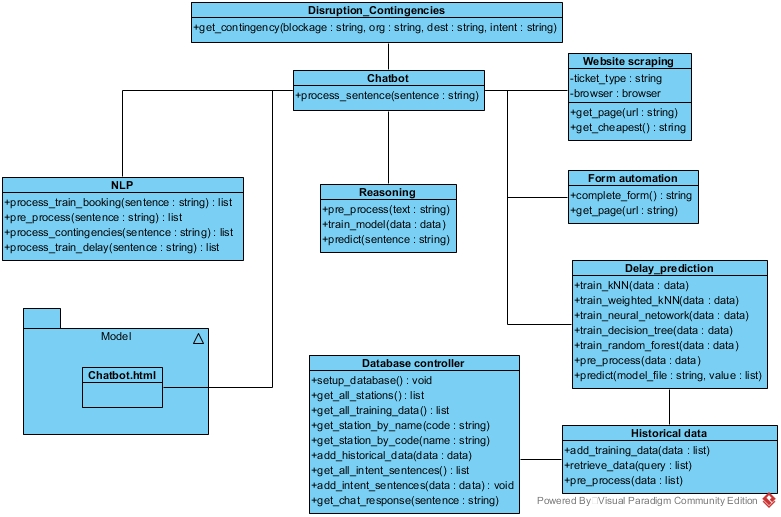
\includegraphics[width=1.0\textwidth]{Chatbot_Structure}
	\caption{Structure of the chatbot }\label{fig:Chatbot_Structure}
\end{figure}
\subsection{User Interface} 
The user interface is created using \textit{HTML} and \textit{CSS} as it provides portability and flexibility during development ans usage. HTML and CSS provides a simple framework for updating and customising the visuals allowing replication of the chatbot across sites with different designs. The user interface is be connected to the back-end using Python \textit{Flask}. While the current plan is to deploy the chatbot online and embedded within a website, existing frameworks such as \textit{Django} and \textit{PhoneGap} can be used to deploy the chatbot across a wider range of platforms. To improve user experience, the current date and time is also printed on the screen. The UI was designed to resemble a physical train ticket to create sense of familiarity to the users.

\begin{figure}[!htb]
	\centering
	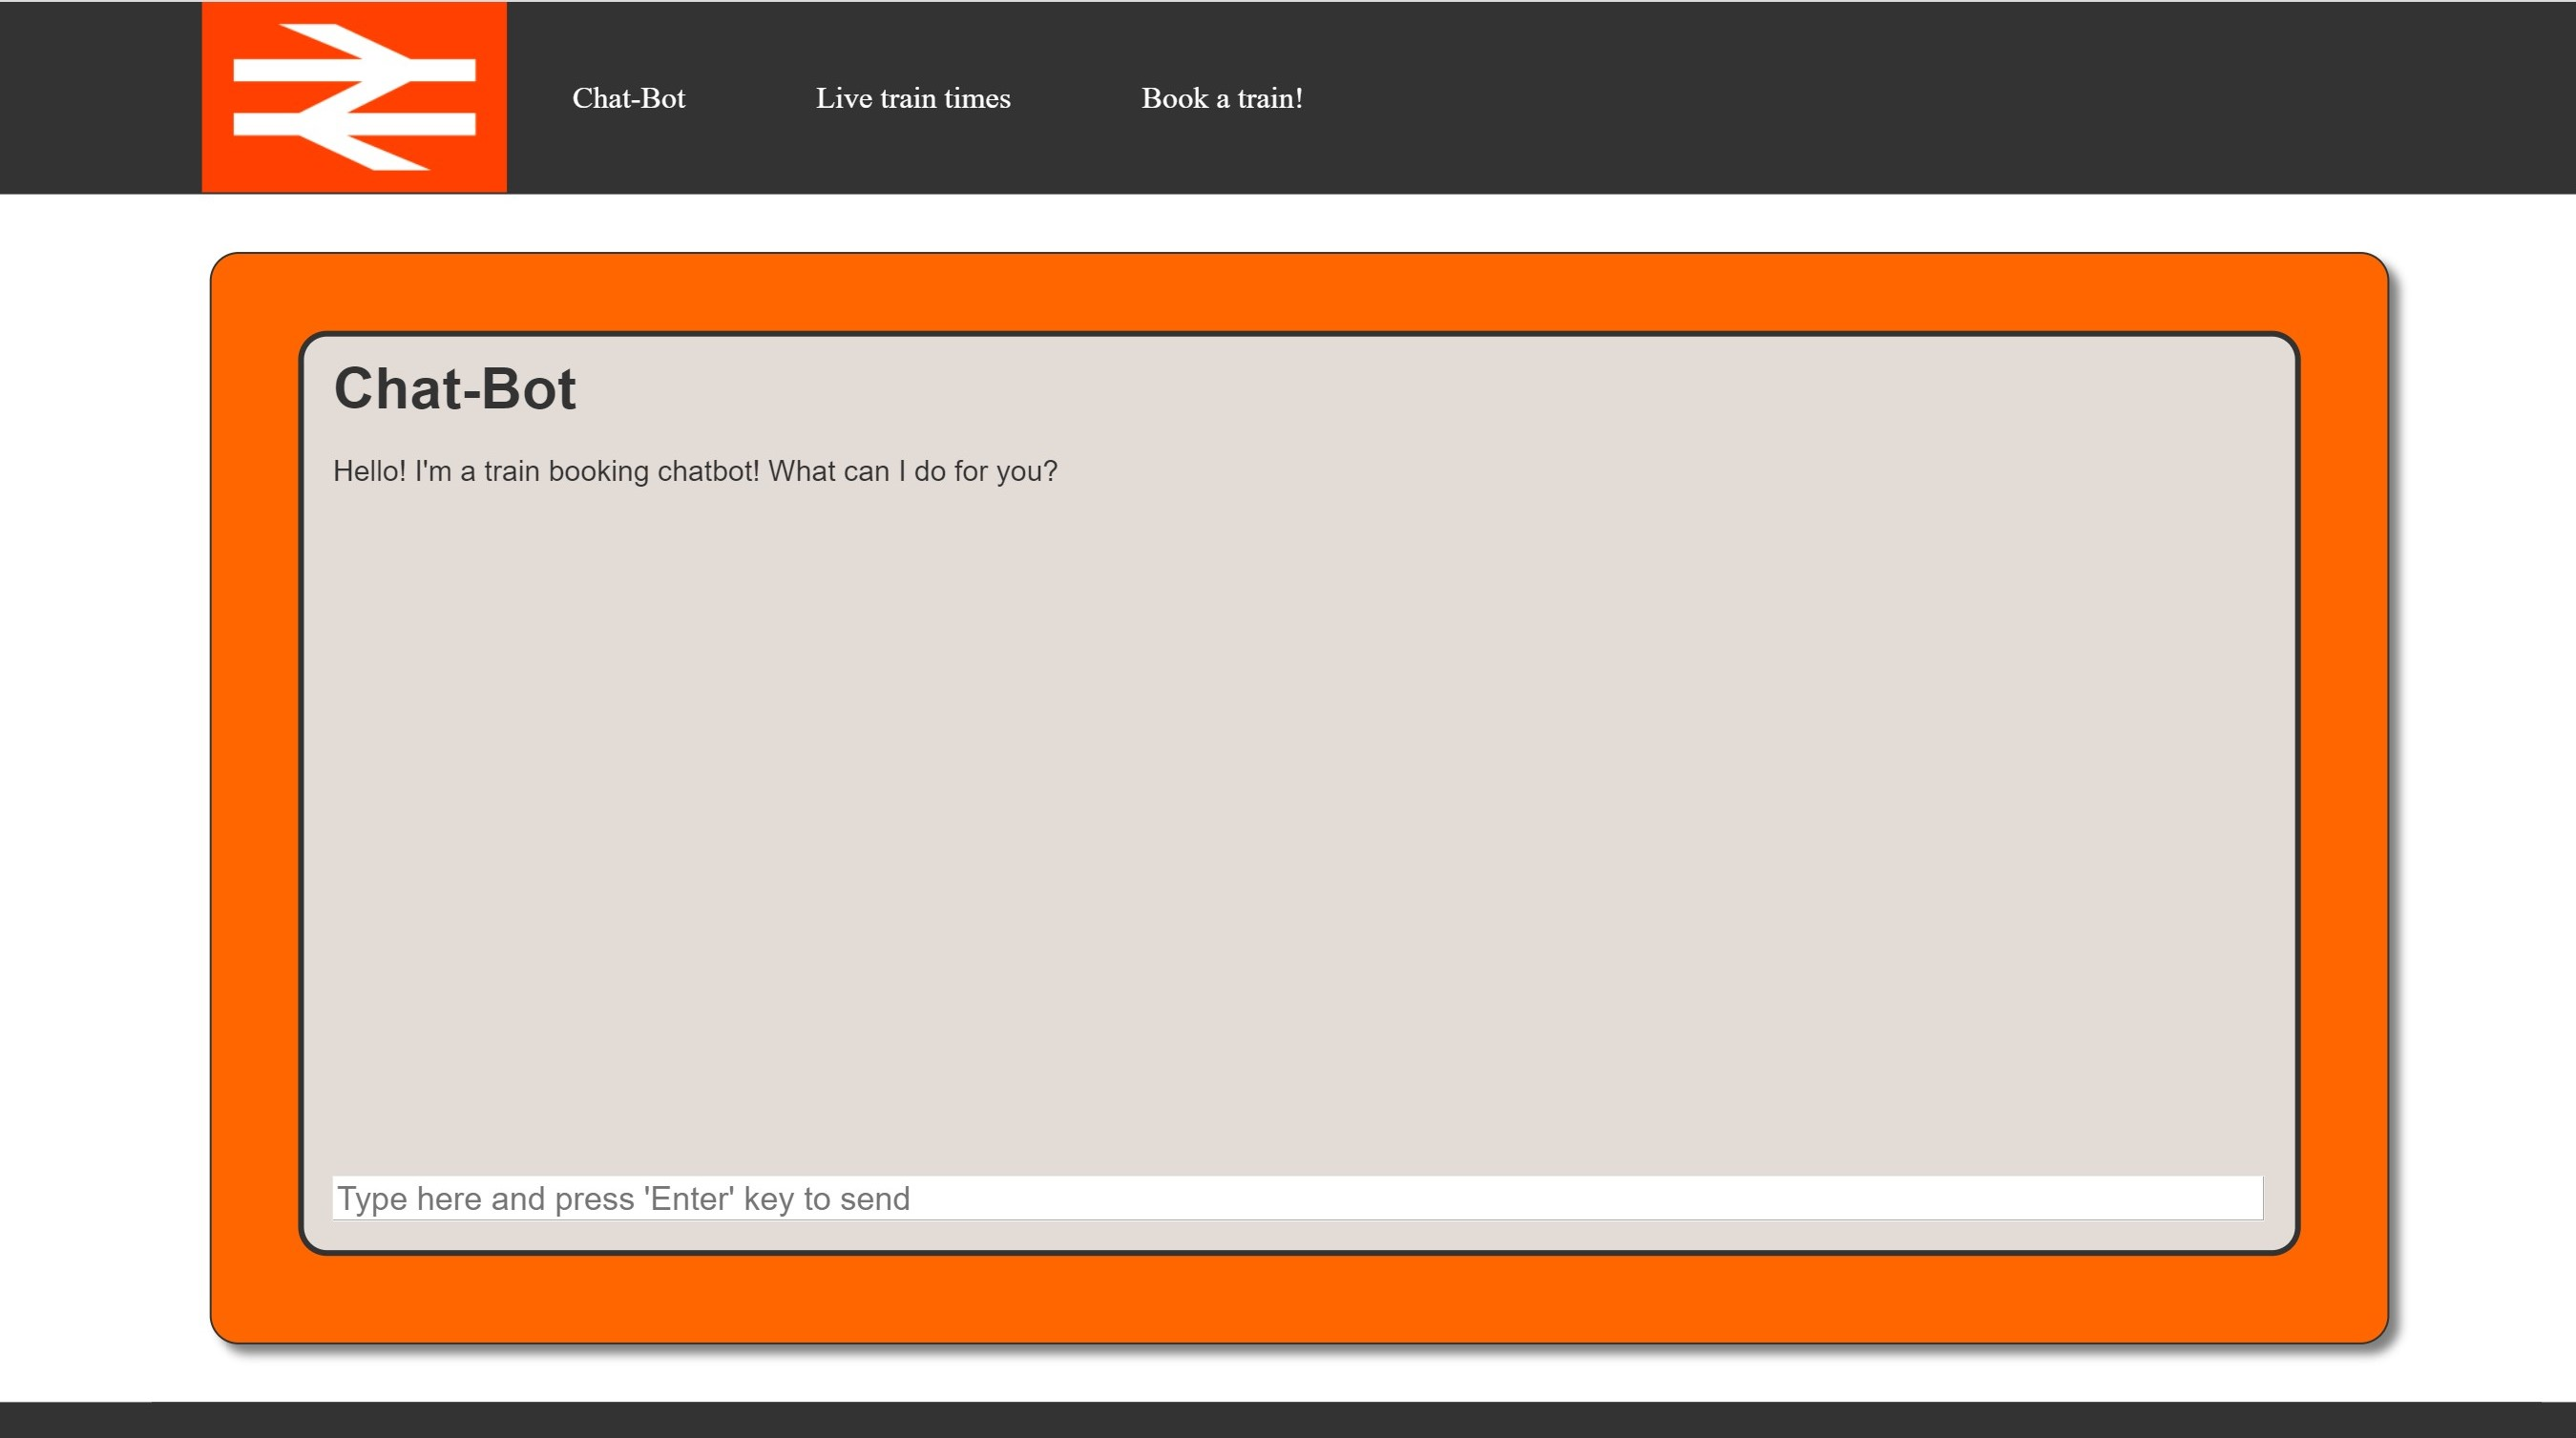
\includegraphics[width=0.9\textwidth]{UI}
	\caption{User interface }\label{fig:UI}
\end{figure}

\subsection{NLP}
Natural language processing mainly rely on the \textit{SpaCy} framework to filter, process and extract required information. The chatbot will also utilise a minor amount of \textit{NLTK} functions to increase the accuracy at which the chatbot picks up the relevant information.

NLP is be the link between the chatbot and background functions that handles train booking, delay prediction and contingency planning. The system extracts information such as location, dates and key words using token tagging and dependencies trained by existing models provided by the framework. Location and date in the sentences is obtained using the entity tagger present in \textit{SpaCy}. Each function will aim to retrieve a set of pre-defined information.

The NLP module can recognise various form of input for date and time. For dates, the natural language processing unit for it can accept dates in the format of \textit{'dd-mm-yy'}, \textit{xxth of Month} and \textit{Month xx}. All formats will be automatically converted to fit the format needed for web-scraping. Aside from that, the date unit will also accept more abstract inputs like "today" or "tomorrow". For the time unit, it will be able to accept "now" as an input in addition to normal 24-hour input.

The methods for information extraction are hierarchical, defined by the specific information it is extracting then grouped by the tasks that the chatbot can accomplish. By designing it this way, a method can not only extract all required information from a single sentence provided that the intent is known and all information is available within the sentence but also extract individual information tokens depending on what's entered in the sentence.

\begin{figure}[!htb]
	\centering
	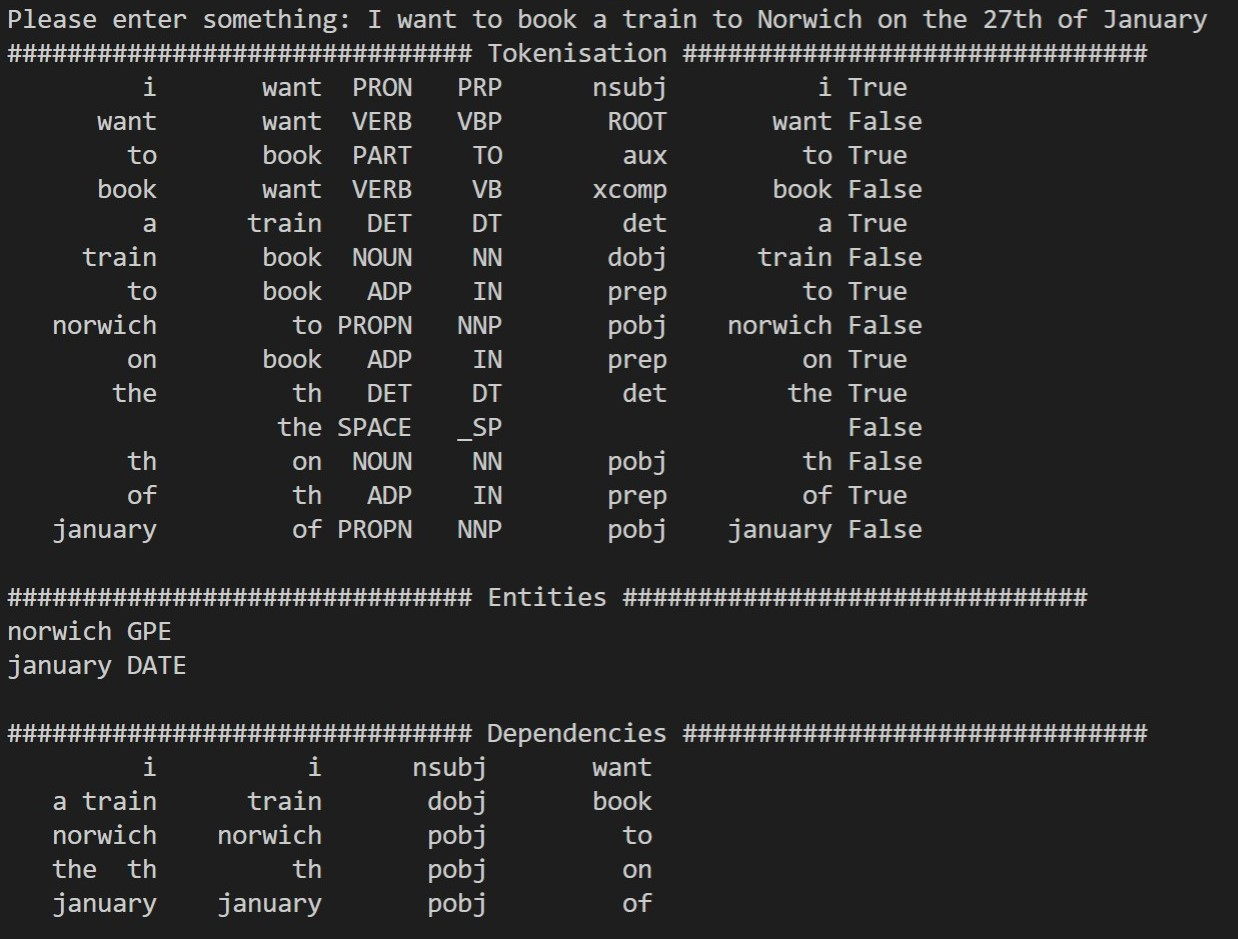
\includegraphics[width=0.7\textwidth]{NLP_Prototype}
	\caption{A prototype of Natural language processing. The system tokenises provided sentence and finds the entities and dependencies }\label{fig:NLP_Prototype}
\end{figure}

Error prevention will also be implemented into the system where spelling mistakes on station names by using trained models to predict the which location is the most likely station that is intended by the user.

\subsection{Reasoning engine}
The reasoning engine was trained using K-nearest neighbours with a database of sentences tagged with intention. The model will be used to predict the intent of sentences entered by users. The sentences will be tagged with '\textbf{B}', '\textbf{C}', '\textbf{D}' and '\textbf{W}' representing \textbf{B}ooking, \textbf{C}ontingencies, \textbf{D}elays and \textbf{W}eather. Additional training data can potentially be added into the database to improve prediction accuracy in the future. The model is trained by vectorising the sentences. The vectors are then hashed to decrease the size to accommodate future growth. As the model predicts by comparing sentence similarity, sentences that contains different location name will still be classified accurately without the need for the specific sentence to be included in the model.

\begin{figure}[!htb]
	\centering
	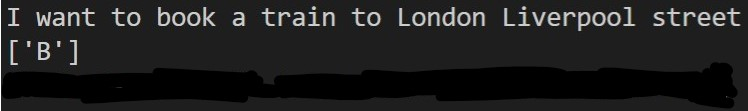
\includegraphics[width=0.7\textwidth]{Reasoning_Prototype}
	\caption{Reasoning engine for the chatbot }\label{fig:Reasoning_Prototype}
\end{figure}

The decision to utilise weighted kNN is to ensure that majority of inputs can be recognised. The model can be constantly updated to adapt to the way user requests for different services. This will allow the system to continue to function efficiently as communication methods change in the future which pre-defined rules might not be able to achieve. As the model predicts by sentence similarity and classifying it by intent, additional intents can be added easily in the future to expand functionality of the chatbot. Additionally, using weighted kNN allows the model to return prediction probability which can be used to ensure that the chatbot will only make decisions above a certain level of confidence.

\subsection{Website scraping}
This module will utilise functions from the \textit{Scrapy}, \textit{BeautifulSoup} and \textit{Selenium} to complete the a booking form and scraping ticket data from the link returned from the form submission. The cheapest train ticket can be retrieved from the list of tickets available and along with the web link, returned to the user for booking. Train ticket information is retrieved from the site \textit{Trainline} by entering auto completing the form using the information collected from conversation with the user and scraping info from the link returned from the form submission. \textit{Scrapy} was later removed from and the detailed explanation can be found in section \ref{Problems}

\subsection{Knowledge-base}
The knowledge-base is be used to store contingencies in the case of railroad disruptions. The module will use the package \textit{Experta}, a new branch of \textit{PyKnow} to define a ruled base inference system to retrieve contingencies. The rules will take the type of blockage (e.g. full or partial) the origin and destination pairs and the type of information the user is requesting. Using these information, the module will then return pre-set contingencies to the user.

For the generation of rules, the information is extracted from the actual contingencies document of train service companies provided for this development. Using the simple rule and fact format of \textit{Experta}, extra rules can be potentially added in the future by staff with limited IT-experience.

\subsection{Prediction Model}
For prediction model, a neural network is used to predict the delays. From analysis of data acquired from \textit{HSP}, we noticed that although the departure delay is available, there isn't a clear connection between the data provided and the delay time therefore a case based reasoning such as kNN might not be able to provide an accurate prediction without the presence of stronger attribute such as delay reason. Additionally, kNN are lazy learners which might significantly increase the prediction time due to the large size of training dataset.

Neural network was considered as the model for delay prediction as multi layer perceptrons aims to create a model that fits the data given instead of finding the training data that fits the unknown data best. Although utilising neural network might result in difficulties when visualising the model however it will produce a better prediction within a shorter time period once the a suitable setting is found.

The model was later modified during implementation with consideration placed on heterogeneous ensembles and a wider range of prediction models. Details are explained in section \ref{Problems}.

\begin{figure}[!htb]
	\centering
	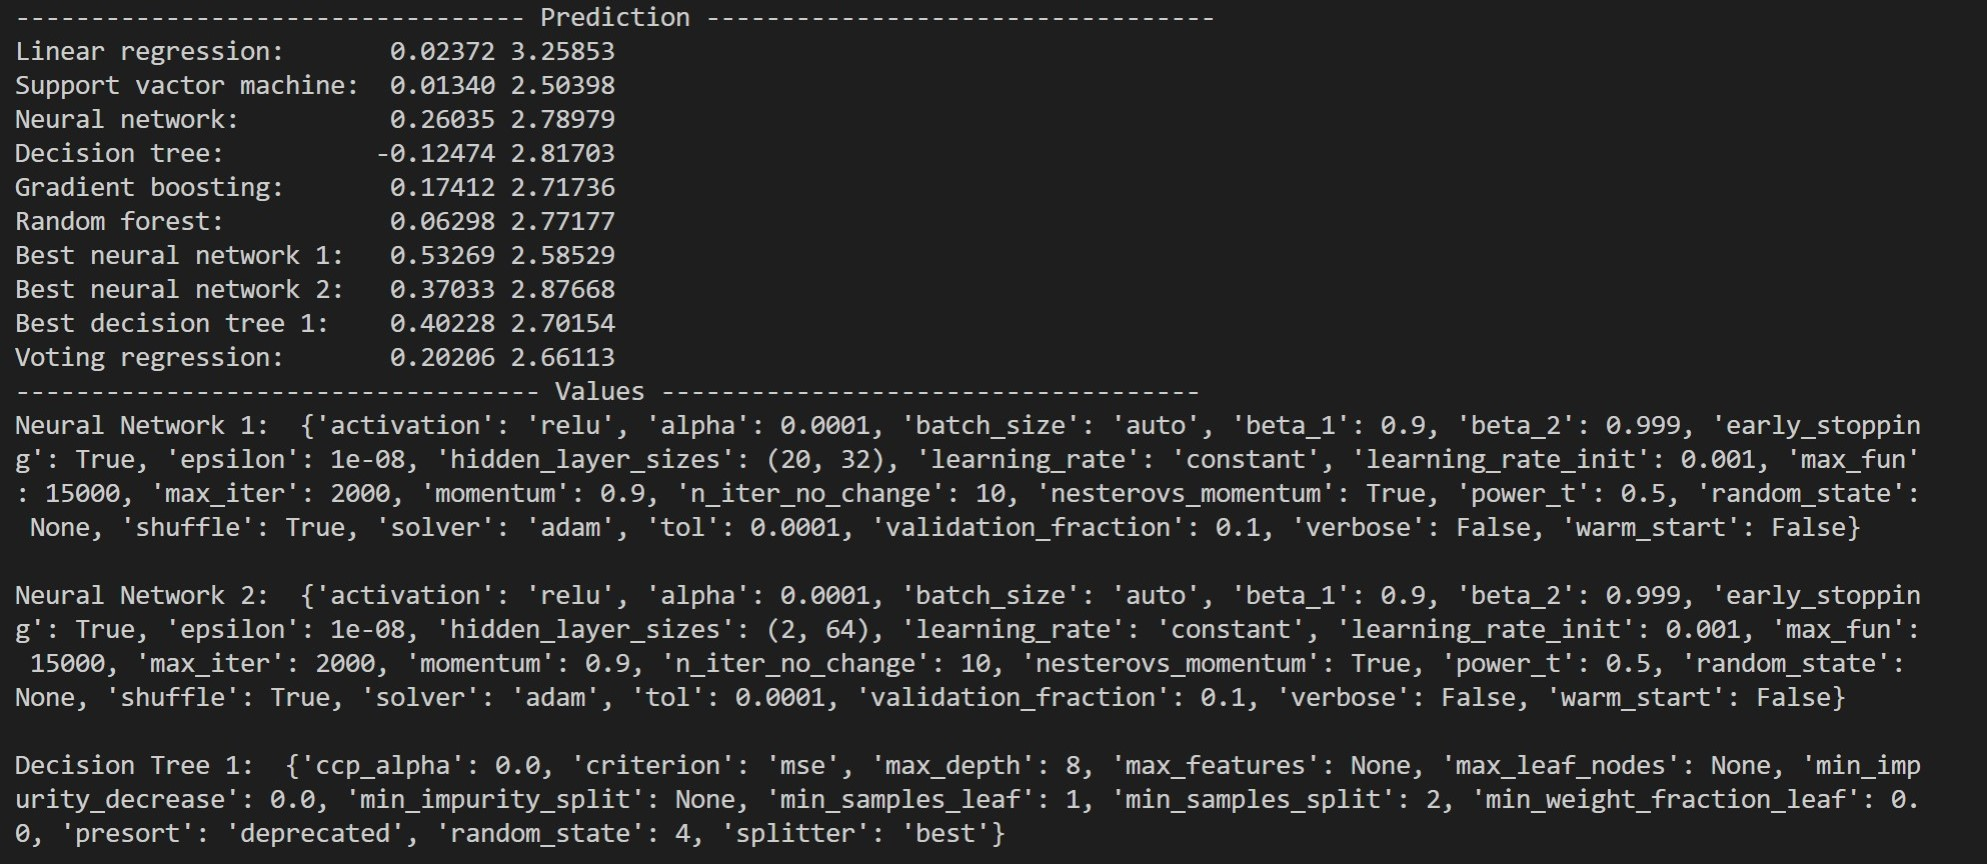
\includegraphics[width=0.99\textwidth]{Prediction}
	\caption{$R^2$ results and mean absolute error of different prediction models. Below shows the parameters of the best models}\label{fig:Prediction}
\end{figure}

\subsection{Data Acquisition}
Data acquisition is designed into the system in two parts. Firstly, historical train data will be acquired, processed and saved into the local database using the \textit{HSP} API which provides data of previous trains and their delays. Historical data can be acquired by providing parameters such as the start and end date of data needed, time and type of day. 3 years of data for trains travelling from Norwich to London Liverpool street will be extracted as the initial dataset for training but the system will allow further addition of data should it be needed. The historical data will contain the following list of information: Origin station, Destination station, Departure time, Departure delay, Arrival time, Arrival delay, Month of year, Type of Date, TOC code. By having Data acquisition built into the system, delay prediction can be expanded in the future to increase the coverage of different train routes. Another consideration during the design of data acquisition was the change of train operating companies or train routes in the future. An example can be seen where there was a new route added from Diss to Hatfield Peverel in 2018 which was not available before. Having in-built data acquisition will improve the ability to update the system without reliance on external software.

Aside from acquiring historical data, the chatbot will also record successful predictions of the user intent to reinforce the model for future predictions. The system will save the initial sentence that was used to determine the intention of the user but will not store the follow up sentences when the system is completing a specific task.

\subsection{Database}
The system database is be created using the package \textit{SQLite}. It will function to store active data that is used by the system which includes: Historical data, Sentence tagged with intent, Responses for normal conversations, Station codes and also a test dataset. These data will be accessed using SQL commands embedded in defined functions within the system. Although using SQL will increase the layers and development work needed for the system, having a database system provides greater flexibility in the way the data can be queried and updated without the need of defining our own methods. It will also provide stronger security as the data saved will not be written in plain files that are easily accessible and understandable by humans which would allow the potential of collecting more personal data in the future if required with a lower level of security concern.

\subsection{Chatbot controller} 
The chatbot controller is the main program that connects all the functionalities together. It accepts input from the UI, processes the sentence using NLP module, predicts intent of the user and completes the task specified. The chatbot uses different agents for each specific tasks. Agents are invoked when the intent is predicted initially and will continue their task until its completion or termination. Current state of the agent is saved in the session cookies and will update according to the pace of the user which allows experienced users to complete tasks faster while also accommodating newer users. This is made possible by the modular information extraction in the NLP modules.

The chatbot controller also accepts sentence training when the intent prediction probability is lower than a certain level. The chatbot will prompt the user to respond with the type of task they were intending with the sentence and update the back-end model according to their response. The controller supports casual conversations where it will reply pre-trained sentences that are not linked to any specific task. Users can also request current weather data of locations by entering sentences regarding to it.

\section{Implementation}
\subsection{Development stages} \label{Dev. stages}
\subsubsection{Stage 1}
During design of the chatbot, dependency analysis revealed that the chatbot relies heavily on the database. Most of the function within the system requires access to the database therefore the development of database is prioritised. Stage 1 focused purely on creating the functions for creation, updating and access of the database. Figure \ref{fig:Stage 1} shows a summary of dependencies between different modules in the system.
\begin{figure}[!htb]
	\centering
	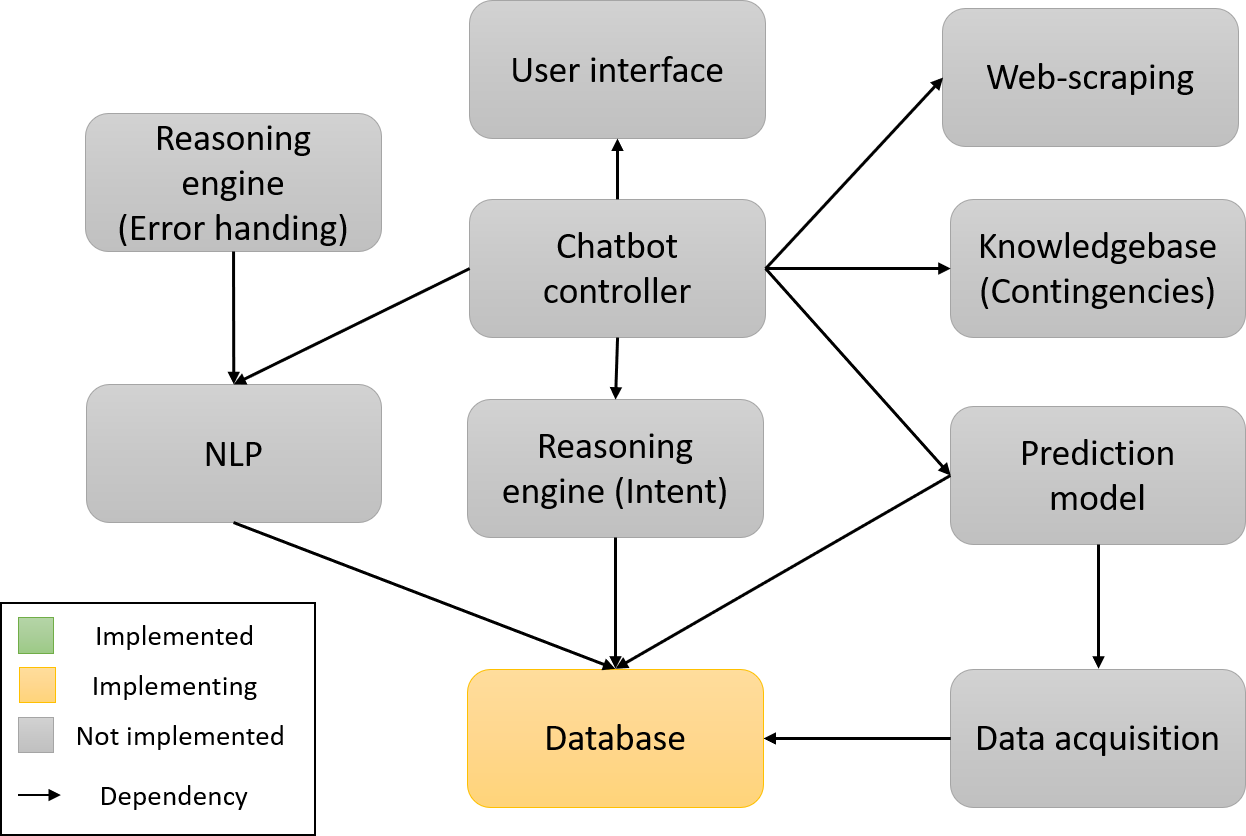
\includegraphics[width=0.6\textwidth]{Stage_1}
	\caption{Stage 1 of Development process }\label{fig:Stage 1}
\end{figure}

\subsubsection{Stage 2}
After development of the database, priority is given to systems that are projected to be time consuming. From analysis of the modules, reasoning engine, natural language processing and data acquisition are chosen to be the modules to focus on for the second stage. 

For the NLP module, having it developed early will allow discovery of how well SpaCy and NLTK discovers entities and dependencies and come up with contingencies if there was any problems during natural language processing. Reasoning engine for intent will also be developed early to ensure that the reasoning engine can accurately predict the intent of sentences by running test on different sentence types. During research, we found out that there are significant amount of historical train data and it will be take time to collect, process and store the data. The prediction module will also take time to test out different type of models and fine tuning the final model however due to its dependency on the data acquisition module the development needs postponed until Stage 3.
\begin{figure}[!htb]
	\centering
	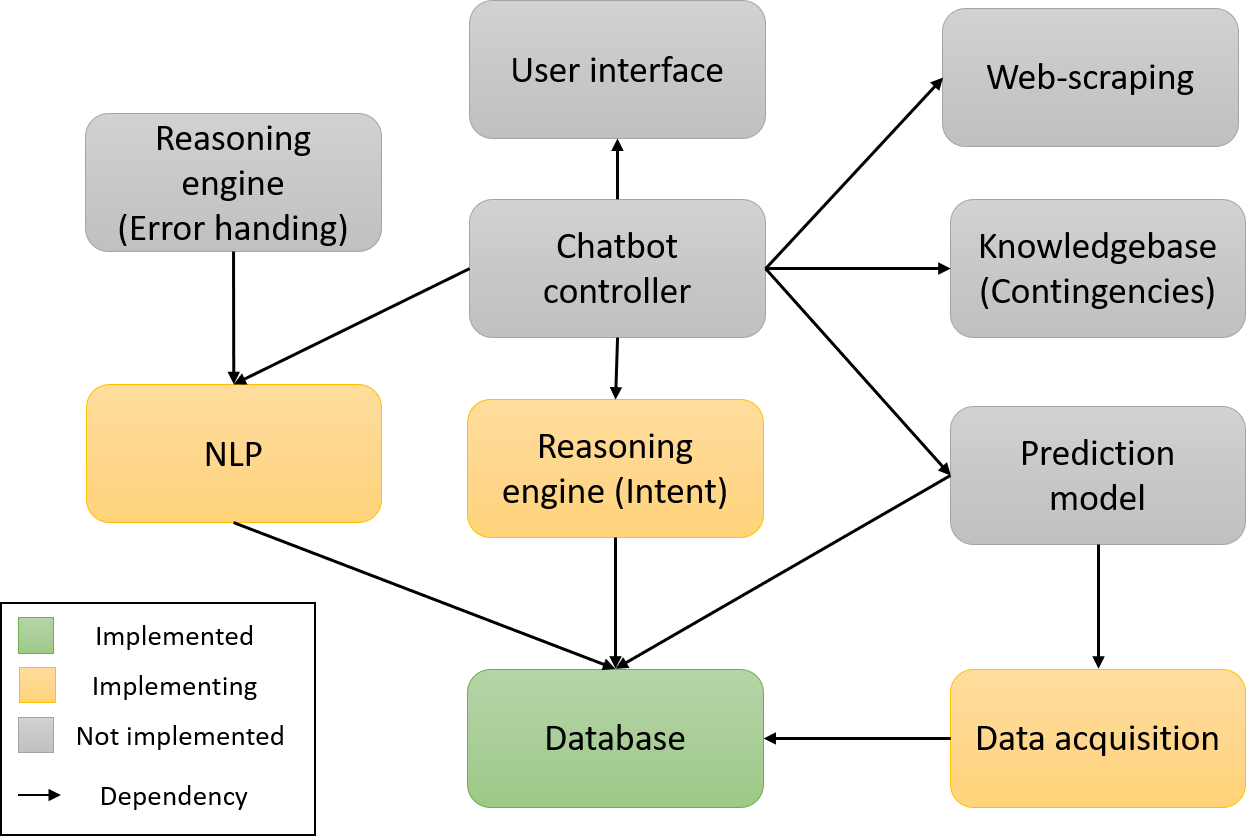
\includegraphics[width=0.6\textwidth]{Stage_2}
	\caption{Stage 2 of Development process }\label{fig:Stage 2}
\end{figure}


\subsubsection{Stage 3}
Stage 3 will focus on the three main functionalities of the chatbot, obtaining cheapest train ticket, providing contingency plans and predicting train delays. For stage 3, the critical task will be the prediction model where large amount of time will be needed for model training and finding the best model to predict delays.
\begin{figure}[!htb]
	\centering
	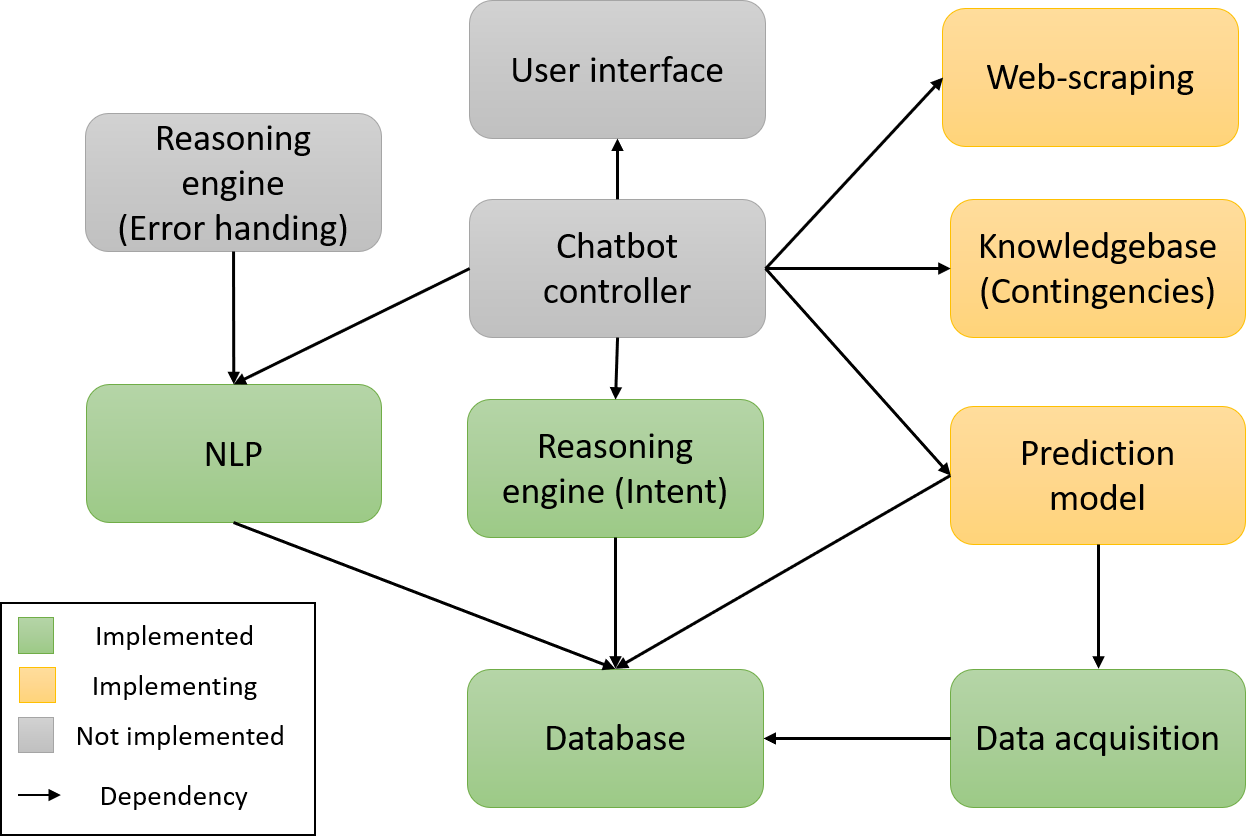
\includegraphics[width=0.6\textwidth]{Stage_3}
	\caption{Stage 3 of Development process }\label{fig:Stage 3}
\end{figure}

\subsubsection{Stage 4}
The focus of stage 4 will be the development of the user interface where the users will be interacting with the chatbot. This stage will also involve the development of basic flask framework that allows communication between the back-end and front-end. During the development of UI, a reasoning engine for error handling in sentences will also be created identify spelling mistakes to improve the usability of the system
\begin{figure}[!htb]
	\centering
	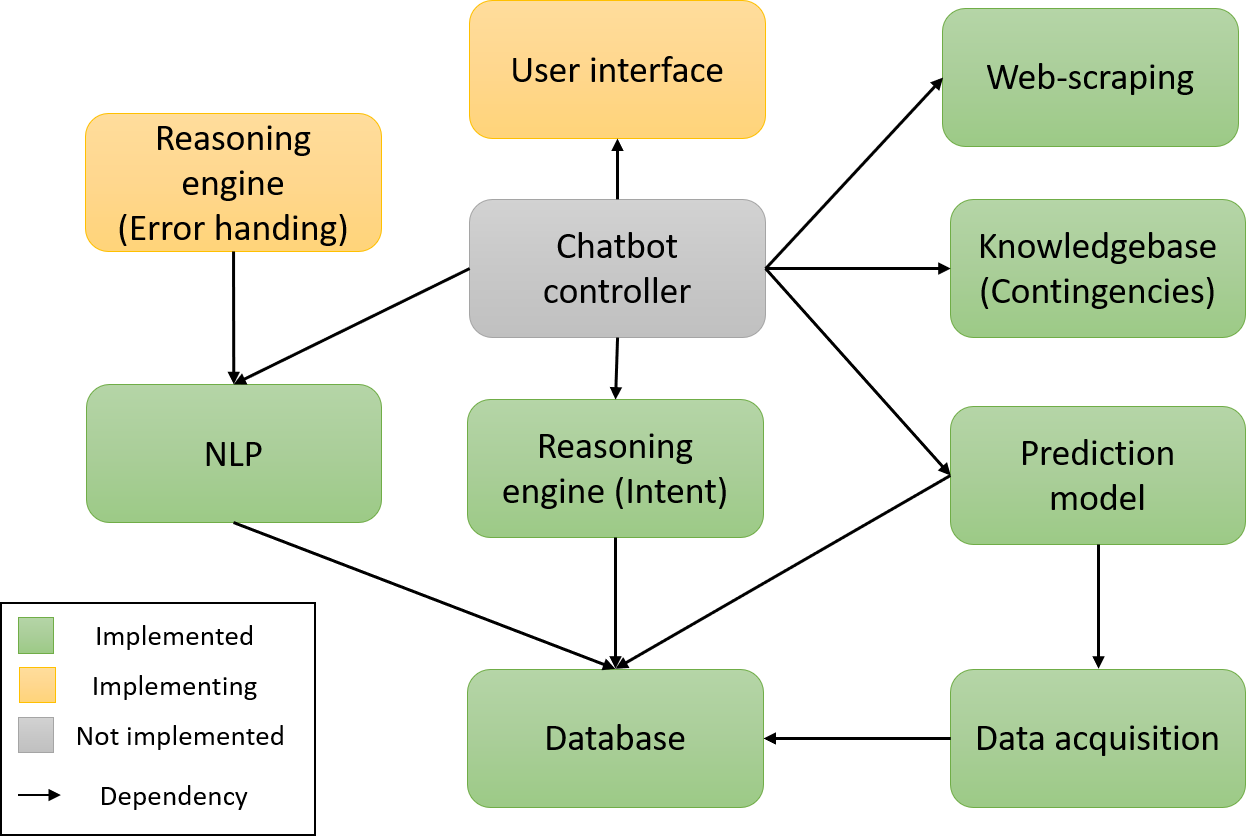
\includegraphics[width=0.6\textwidth]{Stage_4}
	\caption{Stage 4 of Development process }\label{fig:Stage 4}
\end{figure}

\subsubsection{Stage 5}
The final stage will be development of the chatbot controller that connects the flask framework to the python functionalities. Final testing will also be conducted during the stage to ensure that all modules function as expected. 
\begin{figure}[!htb]
	\centering
	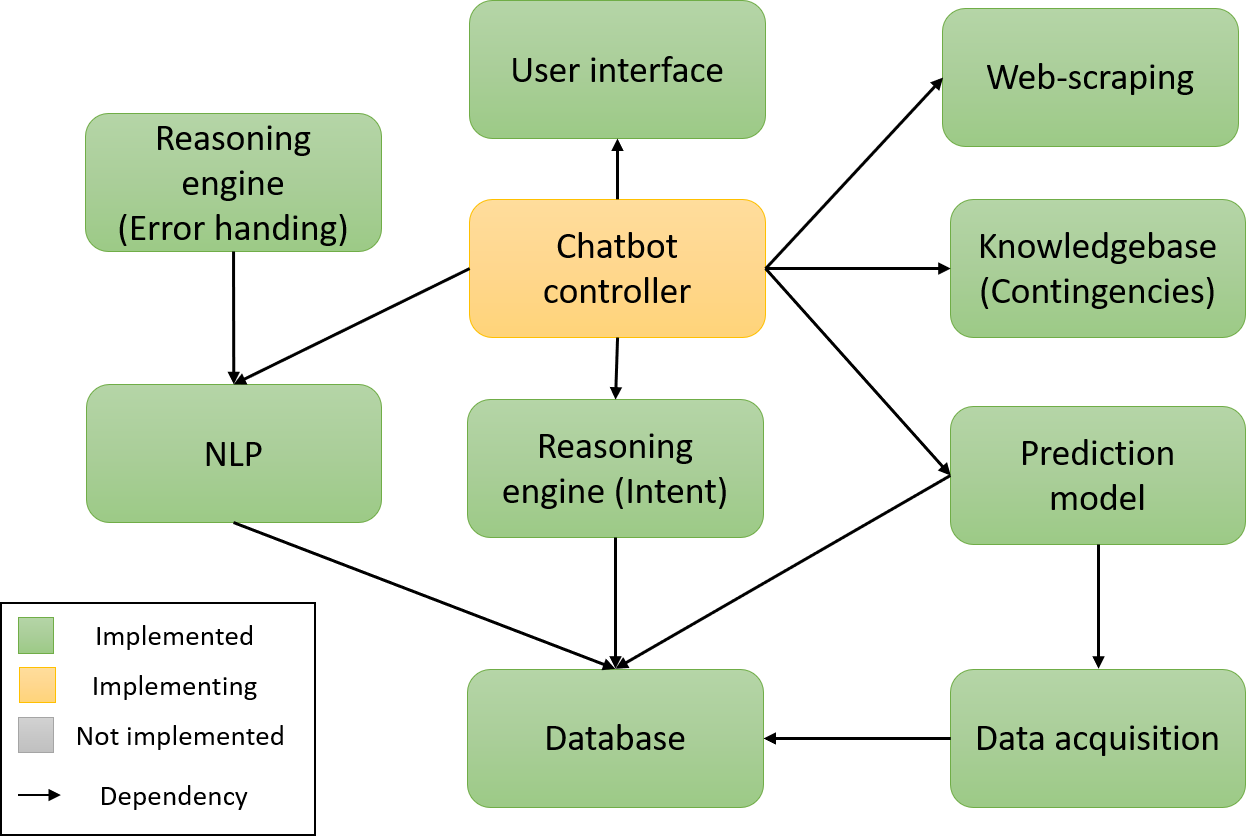
\includegraphics[width=0.6\textwidth]{Stage_5}
	\caption{Stage 5 of Development process }\label{fig:Stage 5}
\end{figure}
\subsection{Problems and Mitigations} \label{Problems}
During development of web scraping module, we found that the ticket data was generated dynamically using JavaScript. As a simple \textit{Scrapy Spider} does not retrieve html data generated dynamically, \textit{Selenium} web driver was used instead to retrieve the full web page and scraped using \textit{BeatifulSoup}.

During evaluation of predictive models, most of models trained with the preset values obtained an extremely low $R^2$ value ($<$ 0.01) and returned highly inaccurate predictions. To improve the accuracy, we defined a list of different values for the settings of the models and by utilising cross validation, obtained the value setting that returns more accurate predictions and a higher $R^2$ of between 0.55 to 0.4 with the prediction accuracy of $+/-2$ minutes. The neural network has 20 hidden layers with constant learning rate and it uses the \textit{adam} solver to find the optimum.

To further address the issue, we modified the system to utilise a heterogeneous ensemble that uses a voting regressor to further improve the prediction accuracy. However, after several test using various combinations of models such as decision trees and support vector machines, the ensemble still scored a lower $R^2$ value compared to the neural network therefore the neural network will be used as the model for delay prediction.

\section{Testing}
Testing is done in different levels of implementation. Firstly, unit testing was done to all the individual modules by writing local main methods to test the functionality and check if it executes and behaves as expected. For modules that depends on input from another, dummy values were provided. These tests will also decrease coupling which will increase the portability of individual modules.

Aside from that, integration testing will be conducted with the completion of a development stage detailed in section \ref{Dev. stages}. These tests focuses on the methods that depends on input from another modules which were previously tested with dummy values during unit testing. This allows early detection of bugs and inconsistencies which can be addressed in an earlier stage of development.

After the system has been assembled, priority will be placed on white-box testing to test all the internal functionalities implemented alongside minor black-box testing to discover potential errors or mistakes. These tests will be monitored and previous working versions will be saved for recovery in case that the testing creates unforeseen irreversible effects. Black box testing was conducted by assigning a tester to test the final product. The tester was given a specification of the chatbot and tasked to discover bugs by interacting with the chatbot in different ways. The discovered bugs was then reported back to the developers and these steps are repeated in an agile development manner. 

\section{Evaluation and Discussion}
\subsection{Contribution}
\begin{itemize}
	\item \textbf{Alvin}  - \textbf{40\%} Main developer for Delay prediction, Web scraping and NLP. Completed report and responsible for bug fixing.
	\item \textbf{Joe}    - \textbf{30\%} Disruption contingencies and testing the chatbot.
	\item \textbf{YuTing} - \textbf{30\%} Part of NLP, prediction model and database. Responsible for video recording and editing for the chatbot.
\end{itemize}

\subsection{Evaluation}
From the testing of the final product, the Chatbot is able to complete the required task to a decent standard. Although there are error prevention and detection in place, extra steps can be taken in the implementation to significantly improve the usability of the chatbot. Further improvements can also be made to increase the types of input the chatbot can accept. Currently, the response provided by the chatbot are simple and generic which can potentially be improved to increase the friendliness of the chatbot.

The design of NLP provides the possibility of expansion due to its modular information extraction. This will allow future expansions such as getting live train data and listing places of interest in a given location. Currently, the prediction models doesn't provide an acceptable accuracy for prediction but through research it was revealed that the cause might be the insufficient significant variables provided. 

Although there are improvements that can be made to this chatbot, we believe the current version is ready for deployment for further testing with clients.

\section{Conclusion or Summary}
Chatbot provides an efficient way to handle common questions and requests and with the introduction of Artificial intelligence and machine learning, The capability of chatbot has significantly improved. Additionally, organisations has begun to put priority in customer engagement which resulted in majority of organisations implementing chatbots on their selected platforms. The opportunity for us to develop a working chatbot prototype allowed to gain insight on the back-end structure of a chatbot which will be incredibly beneficial in this growing industry.

\bibliographystyle{agsm}
%\bibliographystyle{apalike}
% you should use your own bibtex file to replace the following example_ref bib file.
\bibliography{Outline_Ref} 

\end{document}
